\section{Implementation}
In the previous section we introduced the Alpha algorithm and taken assumptions which were transformed into a timed automaton. The former description should be complete enough to implement Alpha algorithm with any suitable tool of choice. In this section we will focus on implementation with regards to the specific tool of our choice, UPPAAL. As the previous section finished on timed automaton, we will start by presenting timed automaton implemented in UPPAAL. We will draw connections between Figure \ref{fig:automaton} and Figure \ref{fig:automaton_uppaal}. Then we will explain global functions and state. Finally, we will outline the limitations imposed on the model by UPPAAL.

\begin{figure}[H]
\caption{UPPAAL implementation of the automaton}
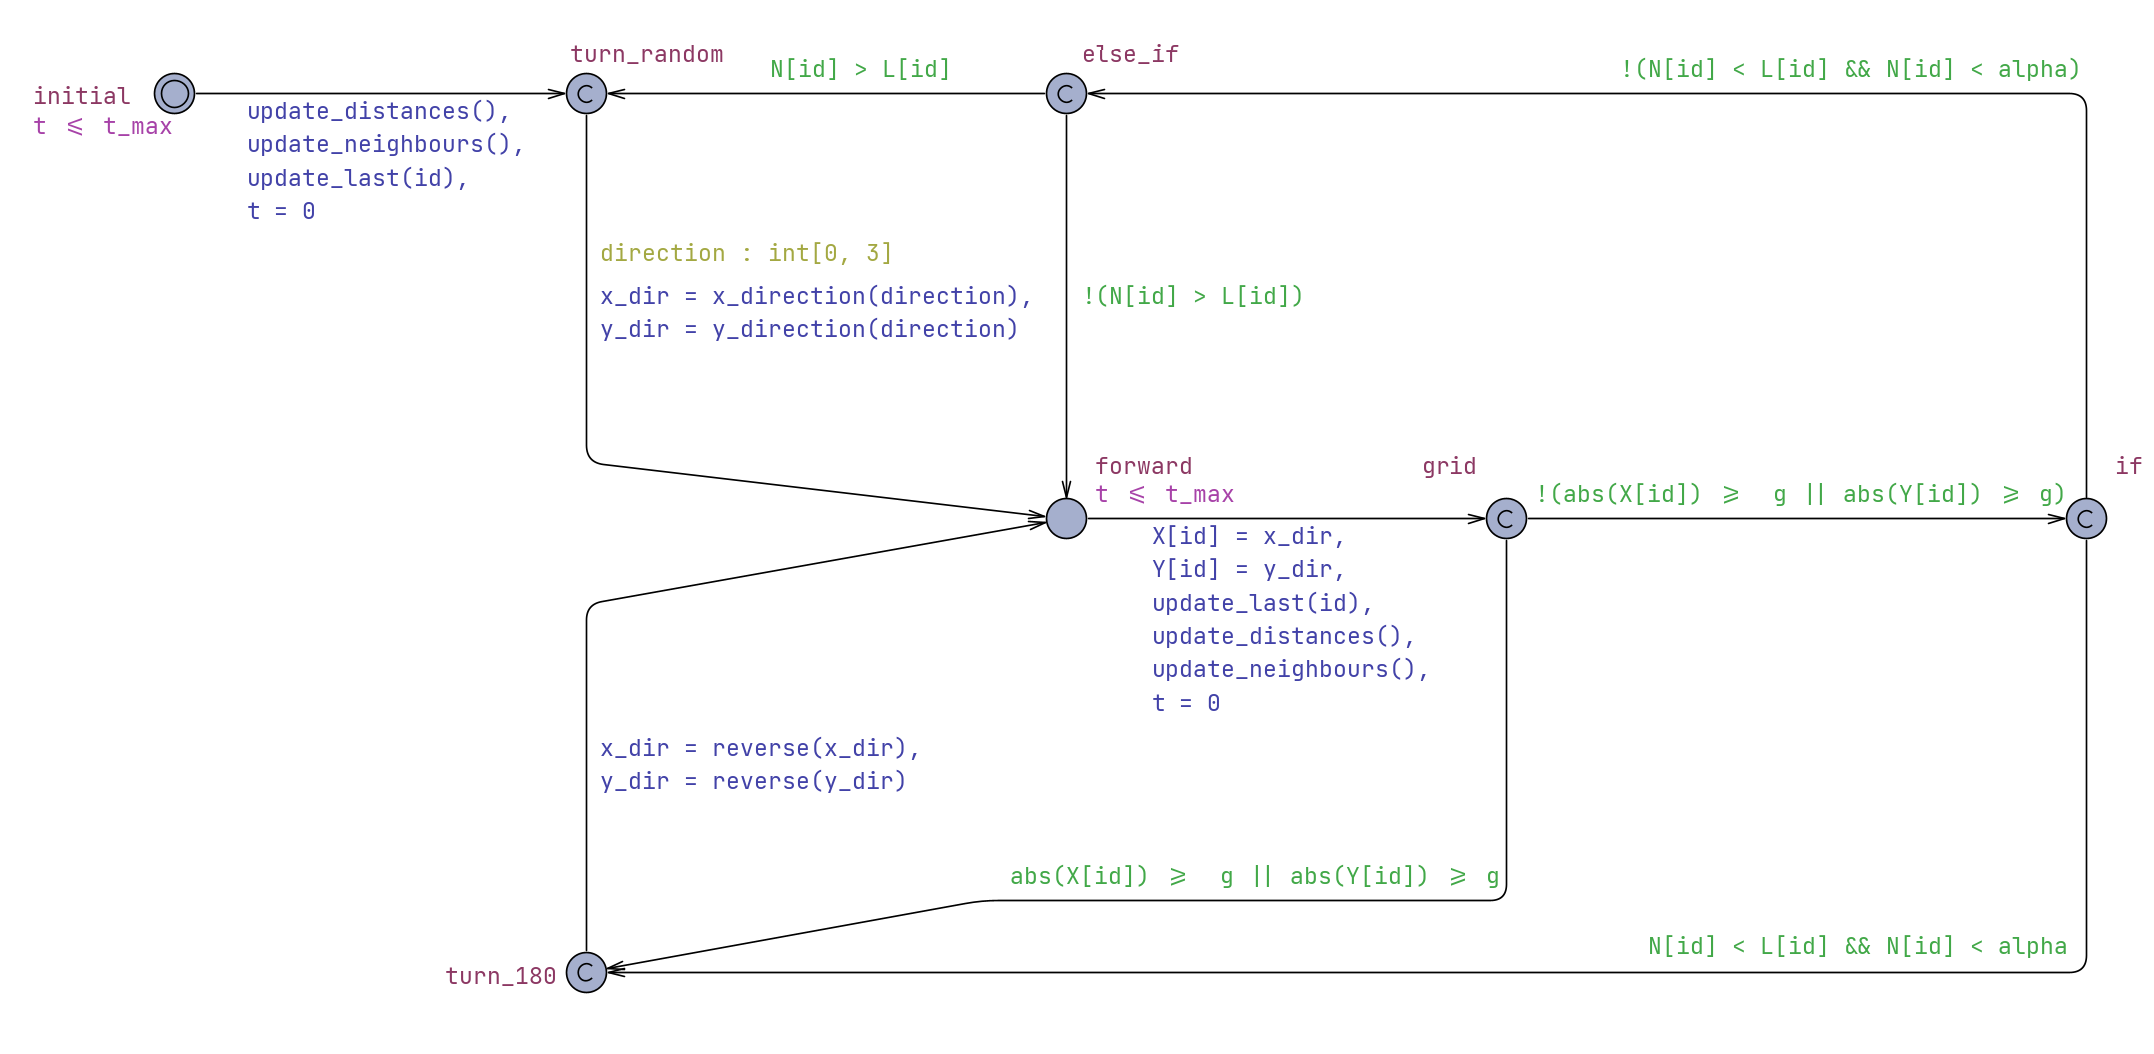
\includegraphics[scale=0.3]{images/automaton_uppaal.png}
\label{fig:automaton_uppaal}
\end{figure}

To start with comparison between general automaton and its specific implementation in UPPAAL, let's notice that both automata have the same set of states and connections. 
